\newcommand{\defs}{../defs}
\documentclass[usenames,dvipsnames]{beamer}

\usepackage[brazilian]{babel}
\usepackage[utf8]{inputenc}
\usepackage{ragged2e}
\usepackage{etoolbox}
\usepackage{multirow}
\usepackage{natbib}
\usepackage{subfigure}
\usepackage{caption}
\usepackage{tikz}
\usepackage{amsmath}
\usepackage{amssymb}
\usepackage{adjustbox}
\usepackage{booktabs}
\usepackage{array}
\usepackage{dot2texi}
\usepackage{minted}
\usepackage{mdframed}
\usepackage{ragged2e}
\usepackage[ruled,vlined]{algorithm2e}

\usefonttheme[onlymath]{serif}

\renewcommand{\thealgocf}{}

\usetheme{Boadilla}
\usecolortheme{seahorse}

\author[Prof. Marcelo de Souza]{}
\date[Udesc Ibirama]{}

\renewcommand{\maketitle}{
	\frame[plain]{
		\titlepage
		\centering
		
		{\scriptsize
			\begin{tikzpicture}[remember picture,overlay,shift={(current page.center)}]
			\node at (-5.7,-4.13) {
\includegraphics[width=.2\textwidth,trim={0 19cm 0 0},clip]{\defs/img/logo-udesc.pdf}};
			\node[align=center]  at (0,-0.4) {%
				\small\textbf{Prof. Marcelo de Souza}\\[3pt]
				\small\texttt{marcelo.desouza@udesc.br}
			};
			\end{tikzpicture}
		}
		
		{\scriptsize
			\begin{tikzpicture}[remember picture,overlay,shift={(current page.center)}]
			\node at (-5.7,-4.13) {
\includegraphics[width=.2\textwidth,trim={0 19cm 0 0},clip]{\defs/img/logo-udesc.pdf}};
			\node[align=left] at (-2.4,-4.11) {%
				\color{black!80}Algoritmos e Estruturas de Dados\\
				\color{black!80}Bacharelado em Engenharia de Software\\
				\color{black!80}Universidade do Estado de Santa Catarina%
			};
			\end{tikzpicture}
		}
	}
}

\addtobeamertemplate{frametitle}{}{%
	\begin{tikzpicture}[remember picture,overlay]
		\node[anchor=north east,xshift=12pt,yshift=2pt] at (current page.north east){
			
\includegraphics[height=1cm,trim={0 19cm 0 0},clip]{\defs/img/logo-udesc.pdf}
		};
	\end{tikzpicture}
}

\addtobeamertemplate{frametitle}{}{\vspace*{-0.5cm}}

\renewcommand{\familydefault}{\sfdefault}

\colorlet{codeboxcolor}{blue!8}

\surroundwithmdframed{minted}

\BeforeBeginEnvironment{mdframed}{}
\AfterEndEnvironment{mdframed}{}

\mdfsetup{%
	backgroundcolor=codeboxcolor,
	linecolor=white}

\setminted{%
	mathescape,
	escapeinside=@@,
	linenos,
	breaklines,
	tabsize=3,
	fontsize=\footnotesize}

\def\arraystretch{1.5}

\captionsetup[figure]{labelformat=empty}
\captionsetup[table]{labelformat=empty}

%\setbeamercovered{transparent}
\setbeamercovered{invisible}

\definecolor{black}{RGB}{0, 0, 0}
\definecolor{darkred}{RGB}{179, 0, 0}
\definecolor{darkblue}{RGB}{0, 0, 51}

\setbeamertemplate{itemize item}{\footnotesize\raise1.25pt\hbox{\color{darkred}$\bullet$}}
\setbeamertemplate{itemize subitem}{\scriptsize\raise1pt\hbox{\color{darkred}$\circ$}}
\setbeamertemplate{itemize subsubitem}{\scriptsize\raise1.5pt\hbox{\color{darkred}$\triangleright$}}
\setbeamertemplate{enumerate item}{\color{darkred}\insertenumlabel.}
\setbeamertemplate{enumerate subitem}{\color{darkred}\insertenumlabel.\insertsubenumlabel}
\setbeamertemplate{enumerate subsubitem}{\color{darkred}\insertenumlabel.\insertsubenumlabel.\insertsubsubenumlabel}

\AtBeginEnvironment{block}{
	\setbeamertemplate{itemize item}{\footnotesize\raise1.25pt\hbox{\color{black}$\bullet$}}
	\setbeamertemplate{itemize subitem}{\scriptsize\raise1pt\hbox{\color{black}$\circ$}}
	\setbeamertemplate{itemize subsubitem}{\scriptsize\raise1.5pt\hbox{\color{black}$\triangleright$}}
	\setbeamertemplate{enumerate item}{\color{black}\insertenumlabel.}
	\setbeamertemplate{enumerate subitem}{\color{black}\insertenumlabel.\insertsubenumlabel}
	\setbeamertemplate{enumerate subsubitem}{\color{black}\insertenumlabel.\insertsubenumlabel.\insertsubsubenumlabel}
}
\AtBeginEnvironment{exampleblock}{
	\setbeamertemplate{itemize item}{\footnotesize\raise1.25pt\hbox{\color{black}$\bullet$}}
	\setbeamertemplate{itemize subitem}{\scriptsize\raise1pt\hbox{\color{black}$\circ$}}
	\setbeamertemplate{itemize subsubitem}{\scriptsize\raise1.5pt\hbox{\color{black}$\triangleright$}}
	\setbeamertemplate{enumerate item}{\color{black}\insertenumlabel.}
	\setbeamertemplate{enumerate subitem}{\color{black}\insertenumlabel.\insertsubenumlabel}
	\setbeamertemplate{enumerate subsubitem}{\color{black}\insertenumlabel.\insertsubenumlabel.\insertsubsubenumlabel}
}

\AtBeginEnvironment{alertblock}{
	\setbeamertemplate{itemize item}{\footnotesize\raise1.25pt\hbox{\color{black}$\bullet$}}
	\setbeamertemplate{itemize subitem}{\scriptsize\raise1pt\hbox{\color{black}$\circ$}}
	\setbeamertemplate{itemize subsubitem}{\scriptsize\raise1.5pt\hbox{\color{black}$\triangleright$}}
	\setbeamertemplate{enumerate item}{\color{black}\insertenumlabel.}
	\setbeamertemplate{enumerate subitem}{\color{black}\insertenumlabel.\insertsubenumlabel}
	\setbeamertemplate{enumerate subsubitem}{\color{black}\insertenumlabel.\insertsubenumlabel.\insertsubsubenumlabel}
}

\let\oldenum\enumerate
\renewcommand\enumerate{\oldenum\justifying}

\let\olditem\itemize
\renewcommand\itemize{\olditem\justifying}

\setbeamertemplate{section in toc}{\color{darkred}\inserttocsectionnumber.~\color{black}\inserttocsection}

\setbeamertemplate{title page}[default][colsep=-4bp,rounded=true]

\setbeamercolor{frametitle}{bg=white}
\setbeamercolor{title}{bg=white}

\setbeamercolor{palette primary}{fg=darkred}
\setbeamercolor{palette secondary}{fg=darkblue}
\setbeamercolor{palette tertiary}{fg=darkblue}
\setbeamercolor{palette quaternary}{fg=darkblue}
\setbeamercolor{normal text}{fg=darkblue}

\setbeamerfont{frametitle}{size=\LARGE}
\setbeamerfont{title}{size=\LARGE}


\setbeamertemplate{footline}
{
	\leavevmode%
	\hbox{%
		\begin{beamercolorbox}[wd=.9\paperwidth,ht=2.25ex,dp=1ex,center]{}%
			\color{black!80} \hypersetup{hidelinks}%
			\insertshortauthor%
			\hspace*{4ex}%
			$\diamond$%
			\hspace*{4ex}%
			\insertshorttitle%
			\hspace*{4ex}%
			$\diamond$%
			\hspace*{4ex}%
			\insertshortdate%
		\end{beamercolorbox}%
		\begin{beamercolorbox}[wd=.1\paperwidth,ht=2.25ex,dp=1ex,right]{}%
			\color{black!80}
			\insertframenumber{} / \inserttotalframenumber\hspace*{2ex}
	\end{beamercolorbox}}%
	\vskip0pt%
}

\setbeamertemplate{navigation symbols}{}

\hypersetup{
	colorlinks,
	linkcolor={black},
	citecolor={blue!80!black},
	urlcolor={blue!80!black}
}

\usetikzlibrary{shapes,arrows,arrows.meta,chains,decorations.pathreplacing,automata,positioning}

\title[Heaps]{Heaps}
\subtitle{Filas de prioridade eficientes}

\immediate\write18{dots/compile.sh heap 0.6 > dots/heap.tex}
\immediate\write18{dots/compile.sh heap 1 > dots/heap2.tex}
\immediate\write18{dots/compile.sh heapify-up1 0.6 > dots/heapify-up1.tex}
\immediate\write18{dots/compile.sh heapify-up2 0.6 > dots/heapify-up2.tex}
\immediate\write18{dots/compile.sh heapify-up3 0.6 > dots/heapify-up3.tex}
\immediate\write18{dots/compile.sh heapify-down1 0.7 > dots/heapify-down1.tex}
\immediate\write18{dots/compile.sh heapify-down2 0.7 > dots/heapify-down2.tex}
\immediate\write18{dots/compile.sh heapify-down3 0.7 > dots/heapify-down3.tex}
\immediate\write18{dots/compile.sh heapify-down4 0.7 > dots/heapify-down4.tex}

\begin{document}

\maketitle

\begin{frame}{Material de consulta}
	\textbf{Leitura obrigatória:}
	\begin{itemize}
		\item Capítulo 2 de~\cite{KleinbergAndTardos2006} -- Análise de algoritmos.
		\begin{itemize}
			\item Seção 2.5 -- Filas de prioridade.
		\end{itemize}
		\item Capítulo 9 de~\cite{GoodrichEtAl2014} -- Filas de prioridade.
	\end{itemize}
	
	\bigskip
	
	\textbf{Leitura complementar:}
	\begin{itemize}
		\item Capítulo 11 de~\cite{Preiss2001} -- Heaps e filas de prioridade.
	\end{itemize}
\end{frame}


\begin{frame}{Revisão de filas de prioridade}
	\begin{itemize}
		\item Estrutura de dados que armazena elementos com suas prioridades.
		\item Operações principais:
		\begin{enumerate}
			\item Inserir elementos.
			\item Recuperar/remover o elemento com maior prioridade.
		\end{enumerate}
	\item Implementação:
	\begin{itemize}
		\item Lista encadeada não-ordenada: operação (2) em $O(n)$.
		\item Lista encadeada ordenada: operação (1) em $O(n)$.
		\item Heap (árvore binária balanceada): todas as operações em $O(\log n)$.
	\end{itemize}
	\end{itemize}
\end{frame}



\begin{frame}{Heaps}
\begin{itemize}
	\item Trata-se de uma árvore binária balanceada.
	\item Os elementos são ordenados de acordo com suas chaves (prioridades).
	\item \textit{Heap order}:
	\begin{itemize}
		\item Para todo nodo $n$, cujo pai é $m$, \texttt{key($m$)} $\le$ \texttt{key($n$)}.
		\item Todo nodo possui maior prioridade (menor chave) que os seus filhos.
		\item Nodos de maior prioridade são armazenados mais acima na estrutura.
	\end{itemize}
\end{itemize}

\begin{figure}
	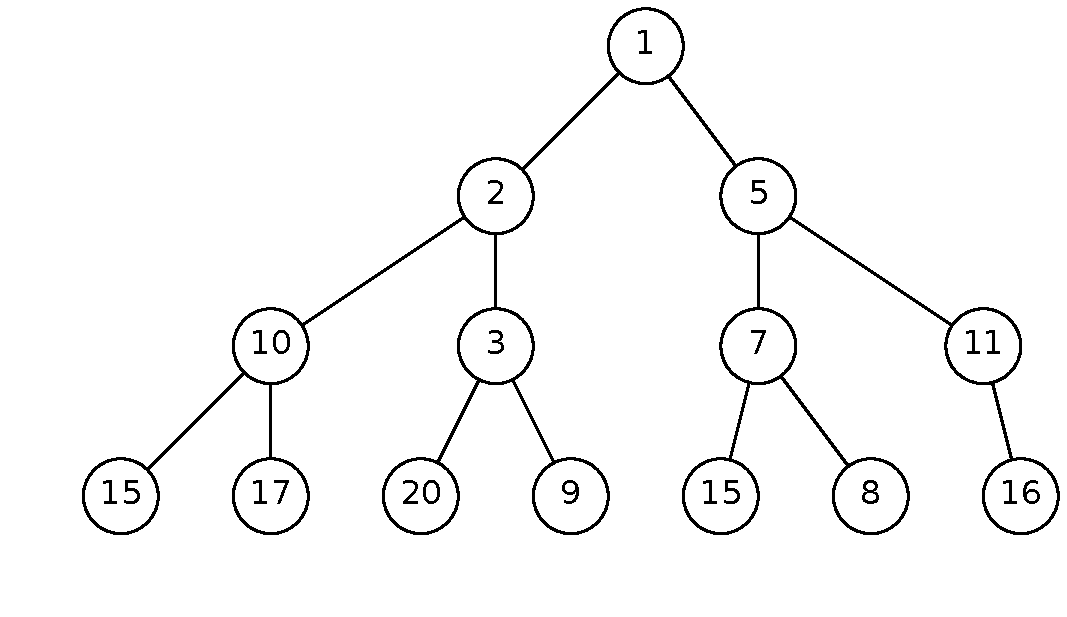
\includegraphics[width=0.6\linewidth]{dots/heap}

\end{figure}
\end{frame}



\begin{frame}{Implementação}
\framesubtitle{Contiguidade -- vetores}
\begin{itemize}
	\item Um vetor armazena todos os elementos da estrutura.
	\item A raiz é armazenada na primeira posição.
	\item Os filhos vão sendo armazenados por níveis na árvore. 
\end{itemize}

\begin{columns}
	\begin{column}{0.48\textwidth}
		\begin{figure}		
			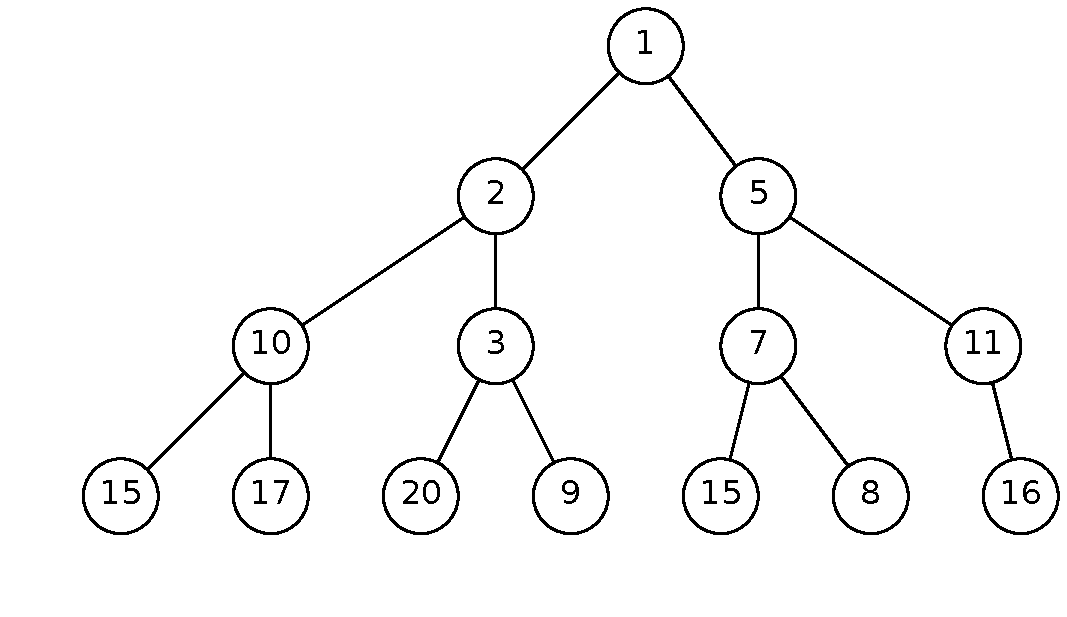
\includegraphics[width=1\linewidth]{dots/heap}

		\end{figure}
		
		\vspace{-30pt}
		
		\begin{figure}
			\scriptsize
			\begin{tikzpicture}[
			start chain = going right,
			node distance = 0pt,
			black,
			cell/.style={draw, minimum width=2em, minimum height=2em, outer sep=0pt, on chain}
			]
			\node [cell] (n1) {1};
			\node [cell] (n2) {2};
			\node [cell] (n5) {5};
			\node [cell] (n10) {10};
			\node [cell] (n3) {3};
			\node [cell] (n7) {7};
			\node [cell] (n11) {11};
			\node [cell] (n15a) {15};
			\node [cell] (n17) {17};
			\node [cell] (n20) {20};
			\node [cell] (n9) {9};
			\node [cell] (n15b) {15};
			\node [cell] (n8) {8};
			\node [cell] (n16) {16};
			\node [cell] (nx) {\#};
			
			\begin{scope}[-{Stealth[length = 2.5pt]}]
			\draw (n1.north) [out=25, in=155] to (n2.north);
			\draw (n1.north) [out=30, in=155] to (n5.north);
			\draw (n2.south) [out=-35, in=-155] to (n10.south);
			\draw (n2.south) [out=-40, in=-155] to (n3.south);
			\draw (n5.north) [out=25, in=155] to (n7.north);
			\draw (n5.north) [out=25, in=155] to (n11.north);
			\end{scope}
			\end{tikzpicture}
		\end{figure}
	\end{column}
	\begin{column}{0.48\textwidth}
		\pause
		\small
		\vspace{-20pt}
		\begin{block}{\small Acesso aos vizinhos na árvore}
			Seja um elemento $i$ da árvore:
			\begin{itemize}
				\item \texttt{leftChild}$(i) = 2i + 1$
				\item \texttt{rightChild}$(i) = 2i + 2$
				\item \texttt{parent}$(i) = \lfloor (i - 1)/2 \rfloor$
			\end{itemize}
		\end{block}
	\end{column}
\end{columns}
\end{frame}



\begin{frame}{Implementação}
\framesubtitle{Detalhes}

\begin{itemize}
	\item Chamamos o vetor de $H$ e sua capacidade de $N$.
	\item Quando a heap tiver $n < N$ elementos, são usados as primeiras $n$ posições do vetor, o que garante o balanceamento da estrutura.
\end{itemize}

\begin{figure}		
	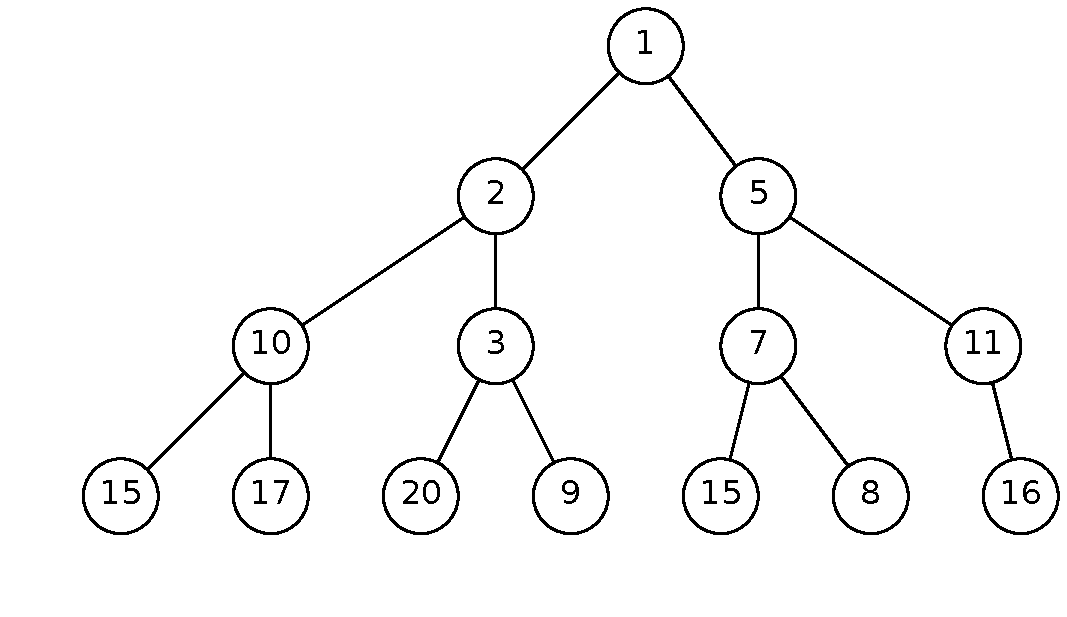
\includegraphics[width=0.6\linewidth]{dots/heap}

\end{figure}

\vspace{-10pt}

\begin{figure}
	\scriptsize
	\begin{tikzpicture}[
	start chain = going right,
	node distance = 0pt,
	black,
	cell/.style={draw, minimum width=2em, minimum height=2em, outer sep=0pt, on chain}
	]
	\node [cell] (n1) {1};
	\node [cell] (n2) {2};
	\node [cell] (n5) {5};
	\node [cell] (n10) {10};
	\node [cell] (n3) {3};
	\node [cell] (n7) {7};
	\node [cell] (n11) {11};
	\node [cell] (n15a) {15};
	\node [cell] (n17) {17};
	\node [cell] (n20) {20};
	\node [cell] (n9) {9};
	\node [cell] (n15b) {15};
	\node [cell] (n8) {8};
	\node [cell] (n16) {16};
	\node [cell] (nx) {\#};
	\node [right = 0.02cm of nx] (nz) {$\dots$};
	
	\begin{scope}[-{Stealth[length = 2.5pt]}]
	\draw (n1.north) [out=25, in=155] to (n2.north);
	\draw (n1.north) [out=30, in=155] to (n5.north);
	\draw (n2.south) [out=-35, in=-155] to (n10.south);
	\draw (n2.south) [out=-40, in=-155] to (n3.south);
	\draw (n5.north) [out=25, in=155] to (n7.north);
	\draw (n5.north) [out=25, in=155] to (n11.north);
	\end{scope}
	\end{tikzpicture}
\end{figure}
\end{frame}



\begin{frame}{Operações heap}
\framesubtitle{Inserção de elemento}

\begin{itemize}
	\item \textbf{Cenário:} adicionar novo elemento $v$ em uma heap $H$ com $n < N$.
	\begin{enumerate}
		\item Insere o elemento na primeira célula vaga $i$ de $H$.
		\begin{itemize}
			\item Isso quebra a propriedade de uma heap.
			\item O elemento adicionado pode ter chave menor que seus ancestrais.
		\end{itemize}
		\item ``Conserta'' a heap com o procedimento \texttt{heapify-up}.
	\end{enumerate}

	\bigskip

	\item \texttt{Heapify-up}: mover o elemento de maior prioridade para cima, até que a propriedade da heap esteja satisfeita.
\end{itemize}
\end{frame}



\begin{frame}{Operações heap}
\framesubtitle{Heapify-up}

\begin{algorithm}[H]
	\DontPrintSemicolon
	
	\If{$i > 0$}{
		Let $j = $ \texttt{parent($i$)} $ = \lfloor (i - 1) / 2 \rfloor$\;
		\If{$key(H[i]) < key(H[j])$}{
			Swap the array entries $H[i]$ and $H[j]$\;
			\texttt{heapify-up(H,\,j)}\;
		}
	}
	
	\caption{\texttt{heapify-up(H,\,i)}}
\end{algorithm}

\vspace{-5pt}

\only<1>{
	\begin{tikzpicture}[remember picture,overlay,shift={(current page.center)}]
		\node [rectangle, align=center, fill=blue!27!white, rounded corners=0.37cm, opacity = 0.75, text opacity = 1, text=black, minimum width=2cm, minimum height=0.7cm, cm={cos(40) ,-sin(45) ,sin(45) ,cos(45) ,(0,0)}] at (2.85, -3.2) {};
	\end{tikzpicture}
	
	\begin{center}
		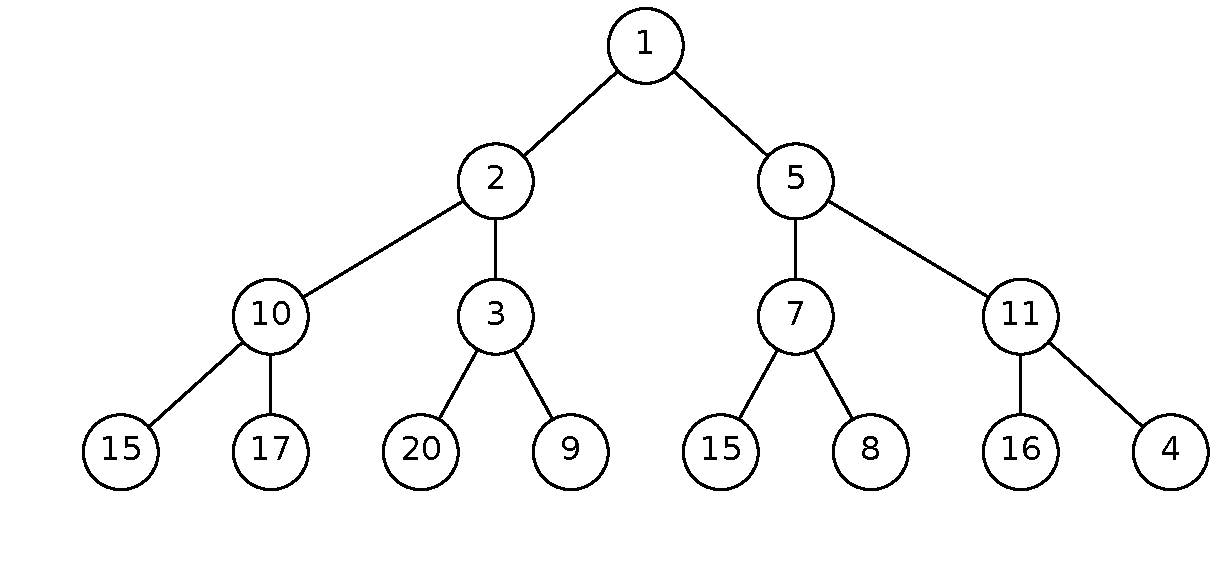
\includegraphics[width=0.6\linewidth]{dots/heapify-up1}

	\end{center}
}

\only<2>{
	\begin{tikzpicture}[remember picture,overlay,shift={(current page.center)}]
		\node [rectangle, align=center, fill=blue!27!white, rounded corners=0.37cm, opacity = 0.75, text opacity = 1, text=black, minimum width=2cm, minimum height=0.7cm, cm={cos(40) ,-sin(45) ,sin(45) ,cos(45) ,(0,0)}] at (2.85, -3.2) {};
	\end{tikzpicture}
	
	\begin{center}
		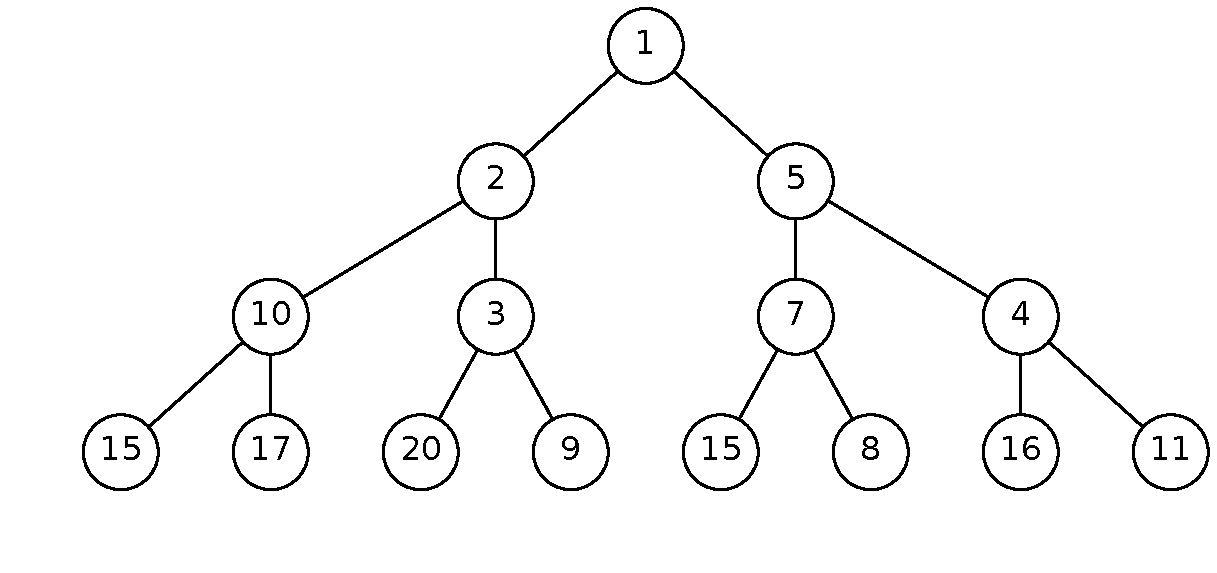
\includegraphics[width=0.6\linewidth]{dots/heapify-up2}

	\end{center}
}

\only<3>{
	\begin{tikzpicture}[remember picture,overlay,shift={(current page.center)}]
	\node [rectangle, align=center, fill=blue!27!white, rounded corners=0.37cm, opacity = 0.75, text opacity = 1, text=black, minimum width=2.4cm, minimum height=0.7cm, rotate=148] at (1.65, -2.32) {};
	\end{tikzpicture}
	
	\begin{center}
		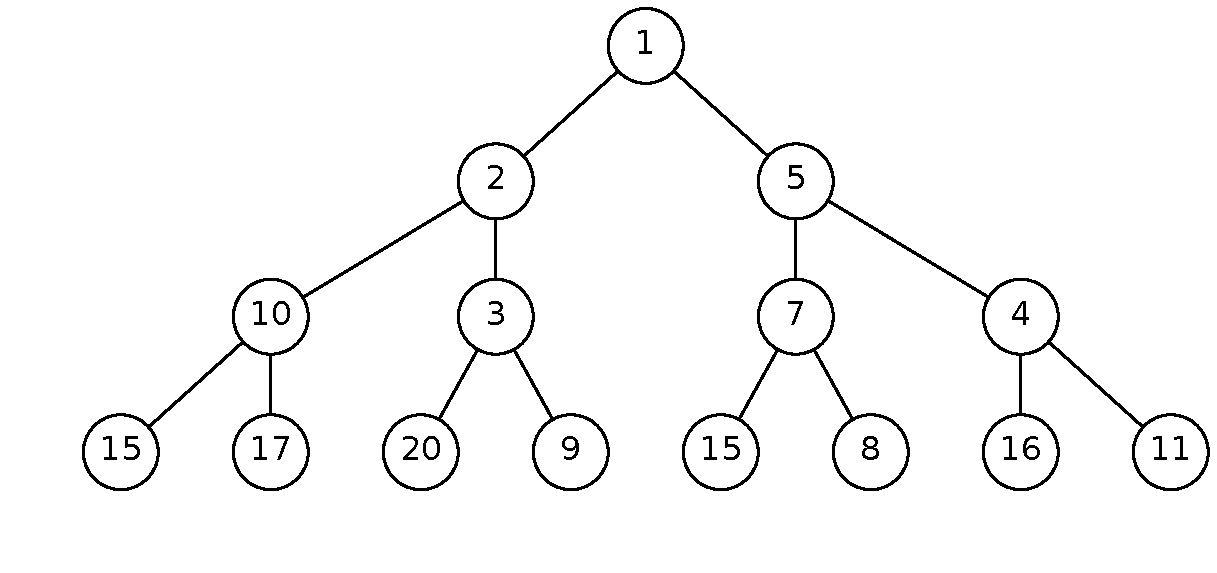
\includegraphics[width=0.6\linewidth]{dots/heapify-up2}

	\end{center}
}

\only<4>{
	\begin{tikzpicture}[remember picture,overlay,shift={(current page.center)}]
	\node [rectangle, align=center, fill=blue!27!white, rounded corners=0.37cm, opacity = 0.75, text opacity = 1, text=black, minimum width=2.4cm, minimum height=0.7cm, rotate=148] at (1.65, -2.32) {};
	\end{tikzpicture}
	
	\begin{center}
		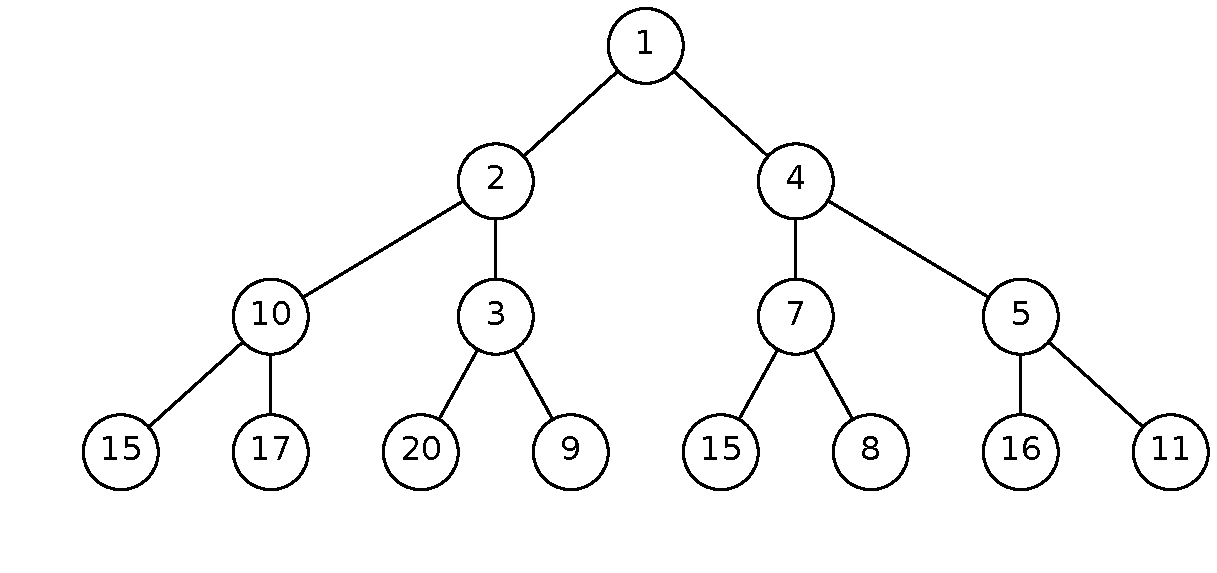
\includegraphics[width=0.6\linewidth]{dots/heapify-up3}

	\end{center}
}

\end{frame}



\begin{frame}{Operações heap}
\framesubtitle{Remoção de elemento}

\begin{itemize}
	\item Em geral, uma fila de prioridades permite a remoção somente do elemento raiz, que possui maior prioridade (operação \texttt{ExtractMin}), mas podemos implementar a remoção arbitrária (operação \texttt{Delete}).
	
	\item \textbf{Cenário:} remover um elemento $v$ em uma heap $H$ com $n$ elementos.
	
	
	\begin{enumerate}
		\item Remove o elemento na célula $i$ de $H$ (posição $H[i]$).
		\begin{itemize}
			\item Isso resulta em um ``buraco'' na árvore.
		\end{itemize}
	
		\item Move o último elemento (folha) da heap para a posição vaga.
		\begin{itemize}
			\item Isso quebra a propriedade de uma heap.
			\item O elemento movido pode ter chave menor que seus ascendentes ou maior que seus descendentes.
		\end{itemize}
		\item ``Conserta'' a heap com o procedimento \texttt{heapify-up} ou \texttt{heapify-down}, conforme a violação criada.
	\end{enumerate}
\end{itemize}
\end{frame}



\begin{frame}{Operações heap}
\framesubtitle{Heapify-down}

\begin{algorithm}[H]
	\DontPrintSemicolon
	
	$n \gets H.size$\;
	\If{$2i + 1 > n$}{
		Terminate with $H$ unchanged\;
	}\ElseIf{$2i + 1 = n$}{
		$j \gets 2i + 1$\;
	}\ElseIf{$2i + 1 < n$}{
		$left \gets 2i + 1$\;
		$right \gets 2i + 2$\;
		$j \gets$ index that minimizes $key[H[left]]$ and $key[H[right]]$\;
	}

	\If{$key[H[j]] < key[H[i]]$}{
		Swap the array entries $H[i]$ and $H[j]$\;
		\texttt{heapify-down(H,\,j)}\;
	}
	
	\caption{\texttt{heapify-down(H,\,i)}}
\end{algorithm}
\end{frame}



\begin{frame}{Operações heap}
\framesubtitle{Heapify-down}

\begin{itemize}
	\item \texttt{Heapify-down}: move o elemento de menor prioridade para baixo, trocando com o menor de seus filhos até que a propriedade da heap seja satisfeita.
\end{itemize}

\only<1>{
	\begin{tikzpicture}[remember picture,overlay,shift={(current page.center)}]
	\end{tikzpicture}
	
	\begin{center}
		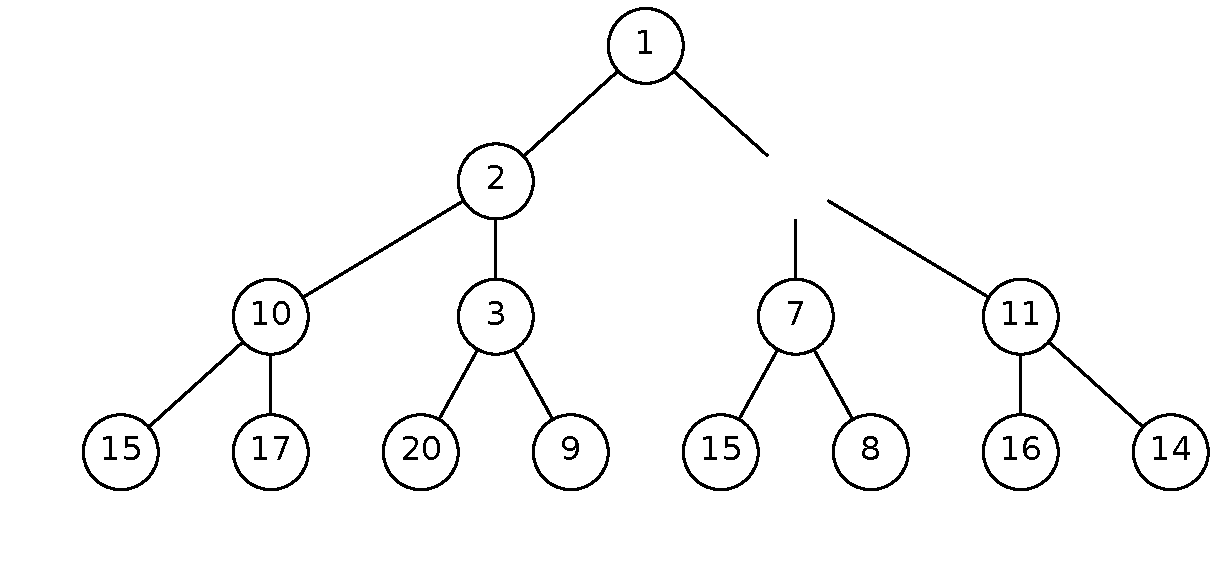
\includegraphics[width=0.7\linewidth]{dots/heapify-down1}

	\end{center}
}

\only<2>{
	\begin{tikzpicture}[remember picture,overlay,shift={(current page.center)}]
		\node [rectangle, align=center, fill=blue!27!white, rounded corners=0.37cm, opacity = 0.75, text opacity = 1, text=black, minimum width=1.8cm, minimum height=0.7cm, rotate=90] at (1.11, -1.68) {};
	\end{tikzpicture}
	
	\begin{center}
		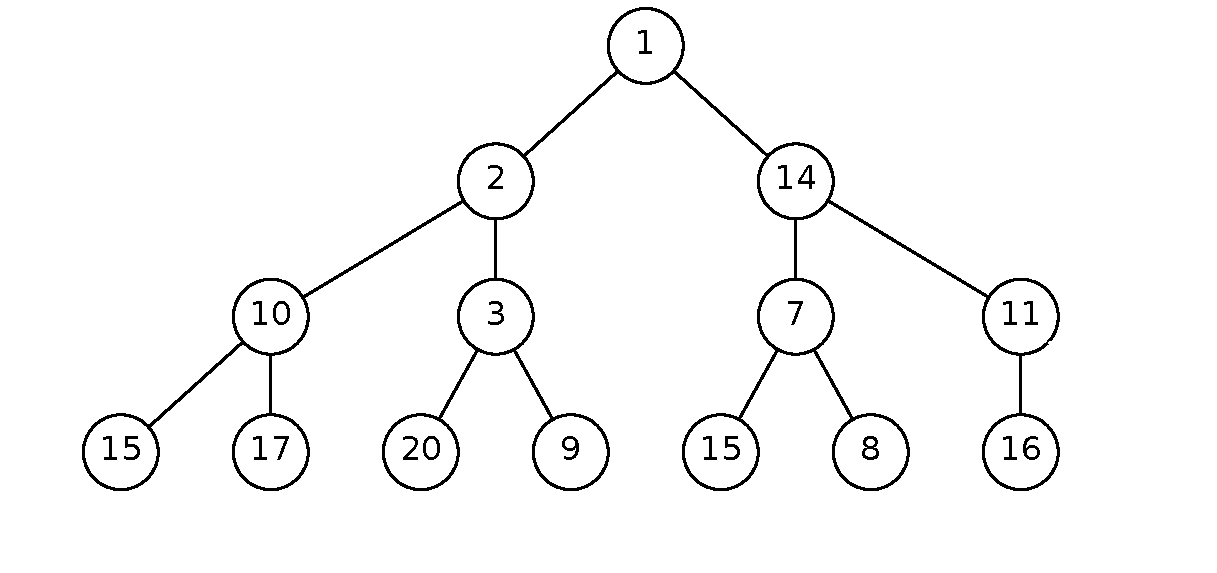
\includegraphics[width=0.7\linewidth]{dots/heapify-down2}

	\end{center}
}

\only<3>{
	\begin{tikzpicture}[remember picture,overlay,shift={(current page.center)}]
		\node [rectangle, align=center, fill=blue!27!white, rounded corners=0.37cm, opacity = 0.75, text opacity = 1, text=black, minimum width=1.8cm, minimum height=0.7cm, rotate=90] at (1.11, -1.68) {};
	\end{tikzpicture}
	
	\begin{center}
		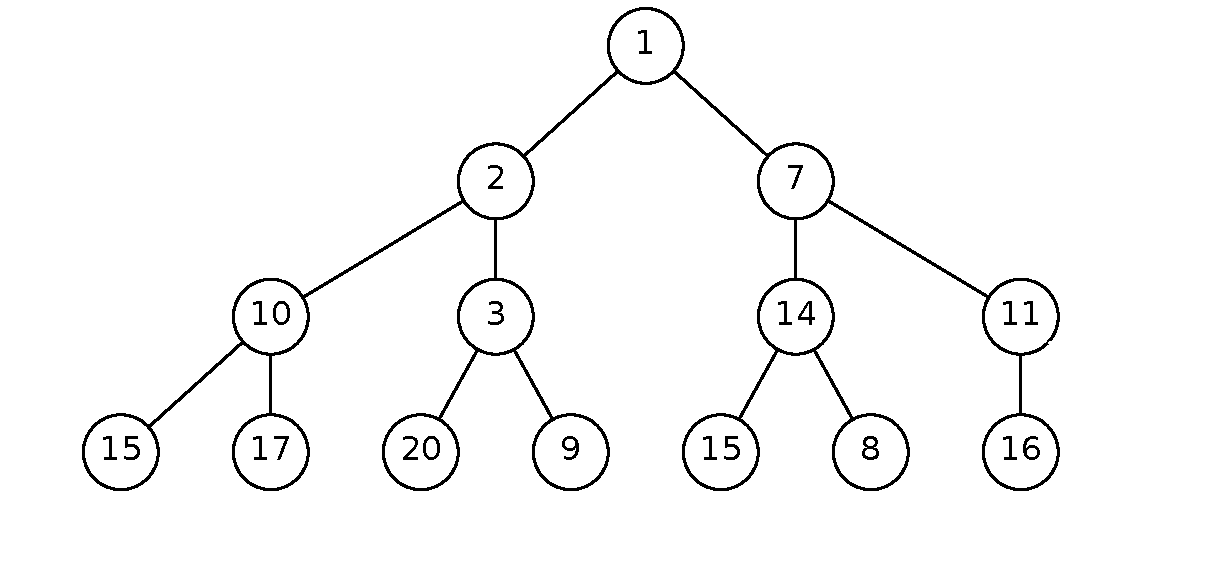
\includegraphics[width=0.7\linewidth]{dots/heapify-down3}

	\end{center}
}

\only<4>{
	\begin{tikzpicture}[remember picture,overlay,shift={(current page.center)}]
	\node [rectangle, align=center, fill=blue!27!white, rounded corners=0.37cm, opacity = 0.75, text opacity = 1, text=black, minimum width=1.9cm, minimum height=0.7cm, rotate=119] at (1.39, -2.68) {};
	\end{tikzpicture}
	
	\begin{center}
		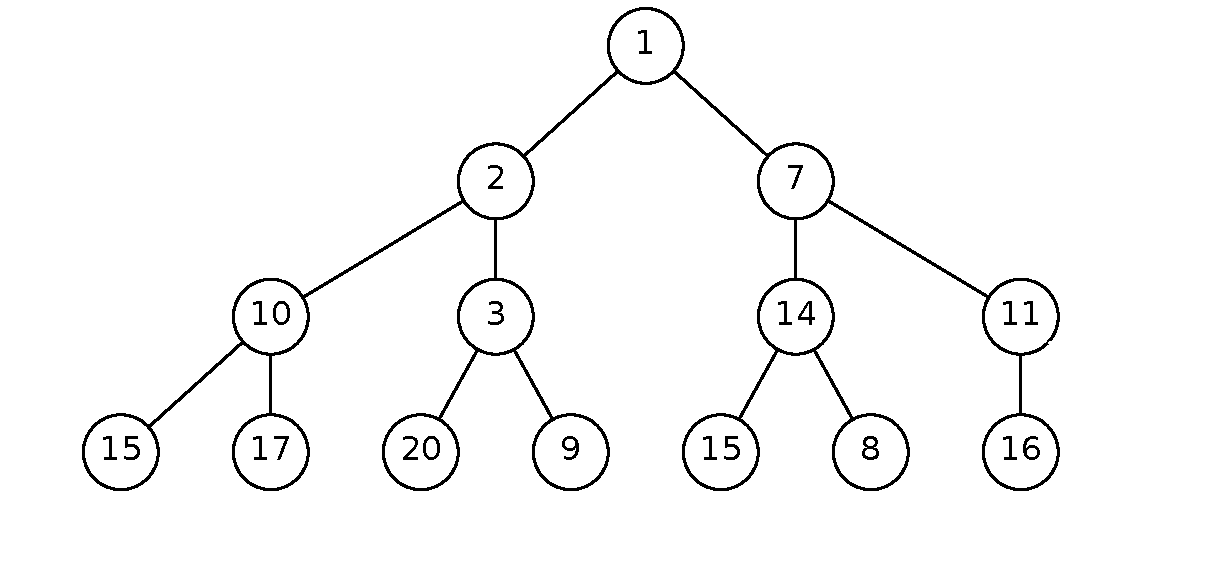
\includegraphics[width=0.7\linewidth]{dots/heapify-down3}

	\end{center}
}

\only<5>{
	\begin{tikzpicture}[remember picture,overlay,shift={(current page.center)}]
		\node [rectangle, align=center, fill=blue!27!white, rounded corners=0.37cm, opacity = 0.75, text opacity = 1, text=black, minimum width=1.9cm, minimum height=0.7cm, rotate=119] at (1.39, -2.68) {};
	\end{tikzpicture}
	
	\begin{center}
		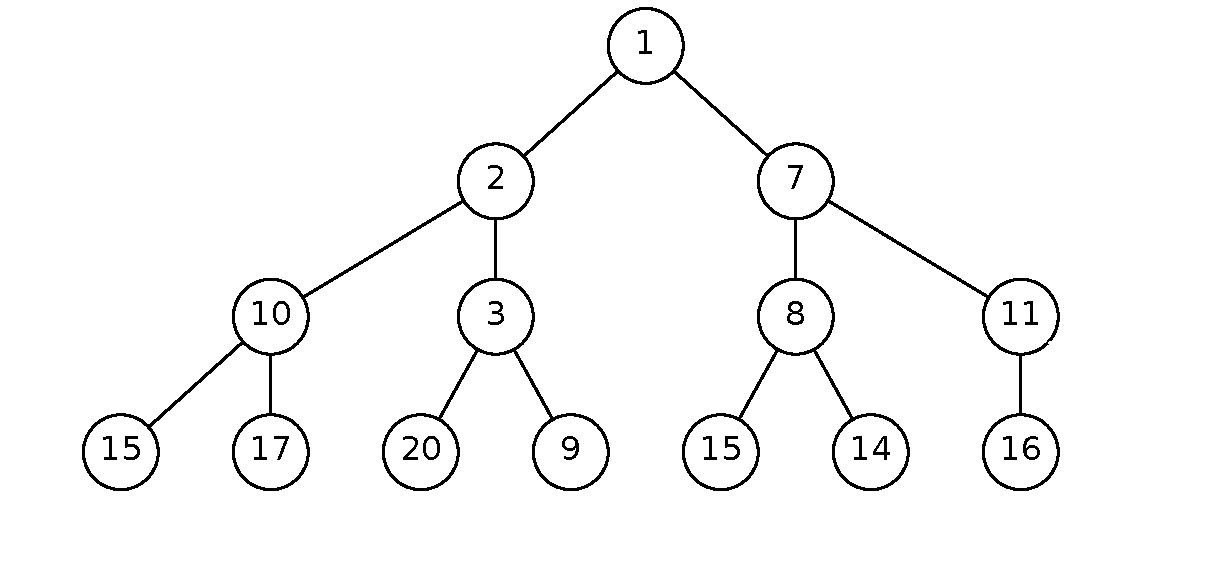
\includegraphics[width=0.7\linewidth]{dots/heapify-down4}

	\end{center}
}

\end{frame}



\begin{frame}{Comparação}
\framesubtitle{Complexidade das operações}

\begin{table}
	\centering
	\begin{tabular}{lccc}
		\hline
		\textbf{Método} & \textbf{Lista não-ordenada} & \textbf{Lista ordenada} & \textbf{Heap} \\
		\hline
		\texttt{size}/\texttt{isEmpty} & $O(1)$ & $O(1)$ & $O(1)$ \\
		\texttt{insert} & $O(1)$ & $O(n)$ & $O(\log n)$ \\
		\texttt{min} & $O(n)$ & $O(1)$ & $O(1)$ \\
		\texttt{removeMin} & $O(n)$ & $O(1)$ & $O(\log n)$ \\
		\hline
	\end{tabular}
\end{table}

\end{frame}


\begin{frame}{Exercício}
\framesubtitle{Implementação com encadeamento}
\begin{enumerate}
	\item Implemente uma heap usando contiguidade para utilizar como fila de prioridades. A estrutura de dados deve fornecer as seguintes operações:
	
	\begin{itemize}
		\item inserir elemento
		\item encontrar o elemento mínimo
		\item extrair elemento mínimo
		\item deletar elemento
	\end{itemize}

	\item Implemente também um método \texttt{changeKey}, que altera a chave (prioridade) de um elemento determinado.
\end{enumerate}
\end{frame}

%\begin{frame}{Atividades}
%	
%\end{frame}

\frame{
	\frametitle{Referências}	
	\setlength{\bibsep}{8pt plus 0.3ex}
	\fontsize{10pt}{10}\selectfont
	\bibliographystyle{apalike}
	\bibliography{../referencias}
}

\end{document}